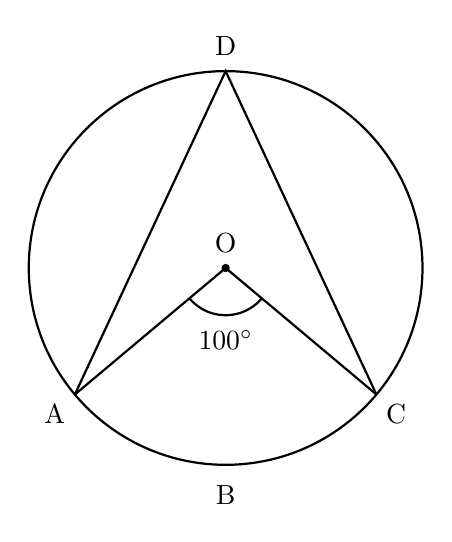
\begin{tikzpicture}[scale=1]

    % Define the radius of the circle
    \def\R{2.5}

    % Define the center of the circle
    \coordinate (O) at (0,0);
    
    % Define points on the circle
    % D is at the top
    \coordinate (D) at (90:\R);
    % A and C are placed such that the central angle AOC is 100 degrees
    % Assuming symmetry around the vertical axis for visual accuracy
    \coordinate (A) at (220:\R);
    \coordinate (C) at (320:\R);

    % Draw the circle
    \draw[thick] (O) circle (\R);

    % Draw the center point
    \fill (O) circle (1.5pt);

    % Draw the segments forming the inscribed and central angles
    \draw[thick] (A) -- (D) -- (C);
    \draw[thick] (A) -- (O) -- (C);

    % Draw the arc indicating the 100 degree central angle
    \draw[thick] (220:0.6) arc (220:320:0.6);

    % Add the labels for the points exactly as shown in the image
    \node[above, yshift=2pt] at (O) {O};
    \node[above, yshift=2pt] at (D) {D};
    \node[below left] at (A) {A};
    \node[below right] at (C) {C};
    
    % Label B is positioned below the circle to denote the arc
    \node[below, yshift=-4pt] at (270:\R) {B};

    % Add the angle measurement
    \node[below, yshift=-2pt] at (270:0.6) {$100^{\circ}$};

\end{tikzpicture}